% Snowflake Data Engineering — Chapter 6 | original manuscript draft
% Author: Arman Golbidi | Editorial snapshot: 22 October 2026
% Compile: xelatex -interaction=nonstopmode -halt-on-error Snowflake_Data_Engineering_Chapter_05.tex
% Trim: 178 x 254 mm; margins inside 23 mm / outside 17 mm / top-bottom 19 mm.
% Body: 10.75 pt / 13.65 pt leading = 1.27 line-height ratio; code: 8.75 pt.
\documentclass[11pt,twoside]{article}
\usepackage[paperwidth=178mm,paperheight=254mm,inner=23mm,outer=17mm,top=19mm,bottom=19mm,headheight=5mm,headsep=4mm,footskip=9mm]{geometry}
\usepackage{fontspec}
\setmainfont{LibertinusSerif-Regular.otf}[BoldFont=LibertinusSerif-Bold.otf,ItalicFont=LibertinusSerif-Italic.otf,BoldItalicFont=LibertinusSerif-BoldItalic.otf]
\setsansfont{LibertinusSans-Regular.otf}[BoldFont=LibertinusSans-Bold.otf,ItalicFont=LibertinusSans-Italic.otf]
\setmonofont{LibertinusMono-Regular.otf}[Scale=0.91]
\usepackage[english]{babel}
\usepackage{microtype}
\usepackage{setspace}
\setstretch{1.0}
\usepackage{titlesec,enumitem,tabularx,array,booktabs,needspace,fancyhdr,lastpage}
\usepackage[most]{tcolorbox}
\usepackage{tikz}
\usetikzlibrary{arrows.meta,positioning,fit,shapes.misc,calc}
\usepackage{listings}
\usepackage{xcolor}
\usepackage{hyperref}
\usepackage{amsmath}
\hypersetup{colorlinks=true,urlcolor=steelblue,linkcolor=steelblue,pdfauthor={Arman Golbidi},pdftitle={Snowflake Data Engineering - Chapter 6: JSON and Semi-Structured Data},pdfsubject={English technical book manuscript, sixth chapter, 178 x 254 mm}}
\definecolor{navy}{HTML}{15334A}
\definecolor{steelblue}{HTML}{17779B}
\definecolor{teal}{HTML}{12888A}
\definecolor{lightblue}{HTML}{ECF5F7}
\definecolor{papergray}{HTML}{F2F5F6}
\definecolor{inkgray}{HTML}{4A5862}
\definecolor{thinrule}{HTML}{CBD7DB}
\AtBeginDocument{\color{navy}\fontsize{10.75}{13.65}\selectfont}
\setlength{\parindent}{0pt}
\emergencystretch=1.3em
\setlength{\parskip}{3.3pt plus 0.7pt minus 0.6pt}
\setlist[itemize]{leftmargin=4mm,itemsep=1pt,topsep=2pt,parsep=0pt}
\setlist[enumerate]{leftmargin=5mm,itemsep=1pt,topsep=2pt}
\titleformat{\section}{\sffamily\bfseries\color{navy}\fontsize{14}{17}\selectfont}{}{0pt}{}
\titlespacing*{\section}{0pt}{8pt}{4pt}
\titleformat{\subsection}{\sffamily\bfseries\color{steelblue}\fontsize{10.8}{13}\selectfont}{}{0pt}{}
\titlespacing*{\subsection}{0pt}{5pt}{1pt}
\newcommand{\topic}[2]{\subsection*{#1\quad #2}}
\newcommand{\repo}[2]{\par\begingroup\fontsize{8.0}{9.6}\selectfont\sffamily\color{inkgray}\textbf{Project reference:} \href{#2}{#1}. \textit{Not independently executed; rights review pending.}\par\endgroup}
\newtcolorbox{insight}[1][]{enhanced,breakable,colback=lightblue,colframe=thinrule,boxrule=.45pt,arc=1.3mm,left=2.8mm,right=2.8mm,top=1.8mm,bottom=1.8mm,before skip=5pt,after skip=5pt,#1}
\newtcolorbox{whitebox}[1][]{enhanced,breakable,colback=papergray,colframe=thinrule,boxrule=.35pt,arc=1mm,left=2.6mm,right=2.6mm,top=1.5mm,bottom=1.5mm,before skip=4pt,after skip=5pt,#1}
\lstdefinestyle{chaptercode}{basicstyle=\ttfamily\fontsize{8.75}{10.7}\selectfont,backgroundcolor=\color{papergray},frame=single,framerule=.35pt,rulecolor=\color{thinrule},breaklines=true,columns=fullflexible,keepspaces=true,showstringspaces=false,aboveskip=5pt,belowskip=5pt,xleftmargin=2mm,xrightmargin=1mm,framexleftmargin=2mm,framexrightmargin=1mm}
\lstset{style=chaptercode}
\pagestyle{fancy}
\fancyhf{}
\fancyhead[LE]{\sffamily\fontsize{7.6}{9}\selectfont\color{inkgray}\textsc{Snowflake Data Engineering}}
\fancyhead[RO]{\sffamily\fontsize{7.6}{9}\selectfont\color{inkgray}\textsc{06 / Semi-Structured Data}}
\fancyfoot[LE,RO]{\sffamily\bfseries\fontsize{8.2}{9}\selectfont\color{steelblue}\thepage}
\fancyfoot[LO,RE]{\sffamily\fontsize{7.6}{9}\selectfont\color{inkgray}Arman Golbidi \quad | \quad Chapter 06}
\renewcommand{\headrulewidth}{0.35pt}
\renewcommand{\footrulewidth}{0pt}
\setcounter{page}{97}
\raggedbottom

% CHAPTER 06 ONLY, pages 97--112 in the planned book
\begin{document}
% page 97 -- chapter opening
{\sffamily\bfseries\fontsize{9}{11}\selectfont\color{steelblue} CHAPTER 06 \hfill DATA ENGINEERING / SEMI-STRUCTURED}\par\vspace{3mm}
{\sffamily\bfseries\fontsize{22}{26}\selectfont\color{navy} JSON and\\Semi-Structured Data}\par\vspace{2mm}
{\sffamily\fontsize{11.3}{14}\selectfont\color{steelblue} Turning changing API payloads into dependable analytical facts}\par\vspace{5mm}
\begin{insight}\textbf{The dashboard did not break. Its meaning did.}\par
At 08:00, the energy dashboard reports the correct daily total. At 09:00, a supplier adds a nested \texttt{unit} field, changes \texttt{observations} to \texttt{measurements}, and represents a missing reading as JSON \texttt{null}. The ingestion job still says \emph{success}. A naive flattening query silently returns zero observations for the new payload. The next chart is empty, not because production stopped, but because the data contract changed.\end{insight}
In Chapter~5, we preserved exact file provenance before accepting source records. This chapter extends the same discipline to nested data. A JSON document is useful because it preserves the source's hierarchy; a data warehouse is useful because it gives that hierarchy consistent analytical meaning. Connecting the two requires more than a cast and a \texttt{FLATTEN}.

\begin{whitebox}\textbf{What you will learn}
\begin{itemize}
\item decide when to retain flexible JSON in \texttt{VARIANT} and when to normalize it;
\item distinguish parse errors, missing paths, JSON \texttt{null}, SQL \texttt{NULL} and wrong types;
\item traverse objects and arrays and reason about the number of rows produced;
\item handle publisher schema revisions without hiding invalid observations;
\item turn mixed-version energy API messages into typed, tested silver-layer records.
\end{itemize}\end{whitebox}
\textbf{Prerequisites.} Chapters~4--5, basic \texttt{SELECT}/\texttt{JOIN}, and familiarity with a JSON object. The companion includes synthetic fixtures and an offline Python validator, requiring no cloud account. Optional Snowflake SQL requires an approved limited role and a small, auto-suspending warehouse. No Snowflake execution or performance benchmark is claimed for this manuscript.

\begin{center}
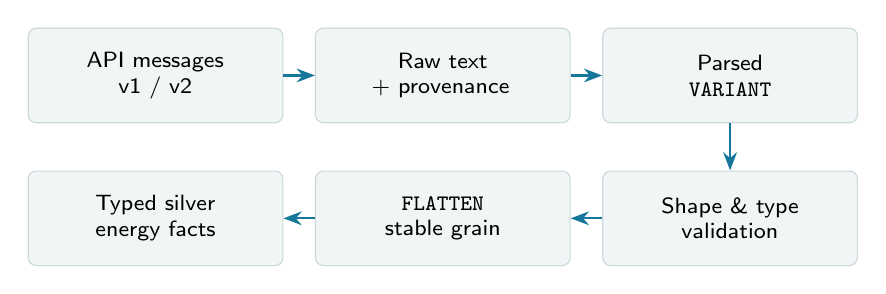
\begin{tikzpicture}[>=Stealth,node distance=4mm,every node/.style={font=\sffamily\fontsize{7.7}{9.3}\selectfont},bx/.style={draw=thinrule,rounded corners=1mm,fill=papergray,text width=30mm,align=center,minimum height=12mm}]
\node[bx] (a) {API messages\\v1 / v2};\node[bx,right=of a] (b) {Raw text\\+ provenance};\node[bx,right=of b] (c) {Parsed\\\texttt{VARIANT}};\node[bx,below=6mm of c] (d) {Shape \& type\\validation};\node[bx,left=of d] (e) {\texttt{FLATTEN}\\stable grain};\node[bx,left=of e] (f) {Typed silver\\energy facts};
\draw[->,thick,steelblue](a)--(b);\draw[->,thick,steelblue](b)--(c);\draw[->,thick,steelblue](c)--(d);\draw[->,thick,steelblue](d)--(e);\draw[->,thick,steelblue](e)--(f);
\end{tikzpicture}\par{\fontsize{8}{10}\selectfont\color{inkgray}Figure 6.1. Preserve the original message while promoting only validated readings.}\end{center}
\newpage
% page 98 -- 6.1 part 1
\section*{6.1\quad Semi-structured data and the VARIANT type}
\topic{6.1.1}{Semi-structured payloads and VARIANT}
A relational table gives each column a declared type and each row an expected shape. API documents often do not. A payload may combine an envelope, a provider identifier, a timestamp, an optional quality flag and a variable number of measurements. Schema variation is not necessarily a data-quality failure: the publisher may be introducing an optional field legitimately. The engineering challenge is to preserve useful flexibility without abandoning predictable outputs.

Snowflake's \texttt{VARIANT} type stores a single semi-structured value, including a JSON-derived object, array, scalar or null. It is not the same as putting opaque JSON \emph{text} into a \texttt{VARCHAR}. Parsing interprets the hierarchy, so queries can navigate paths and work with nested values. Yet the original text may remain important for legal provenance, replay, cryptographic comparison or investigating a parse failure. A robust bronze boundary can preserve both the exact text and a parsed representation, with separate source identifiers.

\begin{lstlisting}[language=SQL,caption={Inspect the type after parsing a synthetic API message.}]
SELECT TYPEOF(PARSE_JSON(
  '{"provider":"synthetic-fi","observations":[{"mwh":12.5}]}'
)) AS document_type;
-- Expected type: OBJECT (illustrative, not cloud-tested).
\end{lstlisting}
The most important distinction is \textbf{schema flexibility versus semantic ambiguity}. A publisher can change the arrangement of fields without altering the meaning of \emph{energy measured during the UTC interval}. But if a field called \texttt{value} changes from MWh to kWh, a successful \texttt{PARSE\_JSON} does nothing to prevent a thousandfold reporting error. Structure and meaning require separate contracts.

\begin{whitebox}\textbf{A two-layer contract}
\begin{itemize}
\item \emph{Envelope contract:} source ID, retrieval time, schema version, valid JSON, payload hash, publisher terms and message identity.
\item \emph{Observation contract:} metric identity, UTC observation time, unit, numeric value, acceptable domain and deduplication key.
\end{itemize}\end{whitebox}
The first contract helps you replay a message accurately; the second tells you which rows should count in a report. Do not confuse storing a document with accepting every measurement it contains. Snowflake's documented guidance permits keeping the flexible structure in \texttt{VARIANT} while promoting high-use attributes into typed columns when workloads are understood.
\repo{P058: Document AI introductory reference}{https://github.com/Snowflake-Labs/sfguide-getting-started-with-document-ai}
\newpage
% page 99 -- 6.1 part 2
\topic{6.1.2}{Parsing types and nested values}
JSON's small type system creates surprisingly large modelling decisions. Its values may be objects, arrays, strings, numbers, booleans or \texttt{null}; it does not define a native timestamp, binary data type or the business meaning of a measurement. The string \texttt{"12.50"} and numeric value \texttt{12.50} may look identical in a dashboard, but a typed transformation should treat them differently until an explicit contract authorizes conversion.

\begin{center}\small\begin{tabularx}{\linewidth}{@{}>{\bfseries}p{33mm}X@{}}\toprule
Incoming form & Example and engineering response\\\midrule
Numeric JSON value & \texttt{12.50}; check range and units before using\\
Numeric string & \texttt{"12.50"}; parse deliberately and record conversion\\
Timestamp string & \texttt{"2026-01-15T10:00:00Z"}; normalize to UTC\\
Object or array & Nested provider information; validate expected structure\\
JSON null & Explicitly supplied null; apply missing-data policy\\
Missing key & No supplied value; distinguish from explicit null\\\bottomrule\end{tabularx}\end{center}

\texttt{TYPEOF} and type predicates help diagnose unexpected values. Consider a measurement property that was a number yesterday but becomes an object with \texttt{amount} and \texttt{unit} keys today. A blind cast may raise an error, or a try-cast may yield SQL \texttt{NULL}. Neither outcome tells the analyst \emph{why} it happened. Your schema-drift report should record the encountered path and type, not simply discard the row.

\begin{lstlisting}[language=SQL,caption={Inspect the nested value before applying a numeric contract.}]
WITH src AS (
  SELECT PARSE_JSON('{"value":{"amount":12.5}}') AS v
)
SELECT TYPEOF(v:value) AS value_kind,
       TYPEOF(v:value:amount) AS amount_kind,
       v:value:amount::VARCHAR AS raw_amount
FROM src;
\end{lstlisting}
The shape \texttt{OBJECT} is expected for the outer \texttt{value}; the inner \texttt{amount} is a number. Cast only after the path and shape have been checked. Native JSON numeric literals may preserve fixed-point values, but the parsing engine can use floating representation for scientific notation or values outside fixed-point bounds. Never infer measurement precision from a screenshot of pretty-printed JSON.

\textbf{Practical judgment.} The bronze schema should not be redesigned every time a nonessential source field appears. The silver schema \emph{should} change through an explicit review whenever a published business metric changes meaning. Keep this separation throughout the book.
\newpage
% page 100 -- 6.1 part 3
\topic{6.1.3}{Choosing schema-on-read versus early normalization}
\emph{Schema-on-read} means preserving a relatively flexible representation and interpreting selected paths when queried. \emph{Early normalization} means parsing, validating and promoting the important attributes into relational columns soon after ingestion. Neither approach is a universal winner. The design should follow the consumer's contract and the likely failure modes.

Use a flexible bronze object when a new source is exploratory, nested fields change frequently, or replay of previously unseen attributes is valuable. Use typed silver columns for stable KPIs, joins, constraints, timestamps and large repeated workloads. In the Finland Energy Analytics platform, bronze retains the provider's JSON, while silver represents one row per \texttt{provider + technology + UTC interval}. An analytical aggregate must never depend on whether the provider called an array \texttt{observations} or \texttt{measurements}.

\begin{center}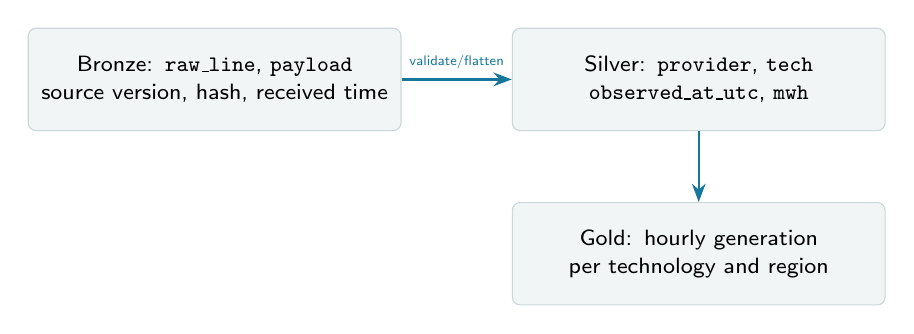
\begin{tikzpicture}[>=Stealth,every node/.style={font=\sffamily\fontsize{8}{10}\selectfont},box/.style={draw=thinrule,fill=papergray,rounded corners=1mm,align=center,text width=45mm,minimum height=13mm}]
\node[box] (b) {Bronze: \texttt{raw\_line}, \texttt{payload}\\source version, hash, received time};
\node[box,right=14mm of b] (s) {Silver: \texttt{provider}, \texttt{tech}\\\texttt{observed\_at\_utc}, \texttt{mwh}};
\node[box,below=9mm of s] (g) {Gold: hourly generation\\per technology and region};
\draw[->,steelblue,thick](b)--node[above]{\tiny validate/flatten}(s);\draw[->,steelblue,thick](s)--(g);
\end{tikzpicture}\par{\fontsize{8}{10}\selectfont\color{inkgray}Figure 6.2. Promote a well-defined business grain, not an accidental JSON shape.}\end{center}

A less obvious issue is \emph{reprocessing}. A schema correction might require recreating a silver table from last week's original messages. If bronze keeps only a destructive transformation and discards the payload, the repair may be impossible without retrieving the source again. Preserving exact source text and publishing a migration plan makes that recovery feasible.

\begin{insight}\textbf{Decision rule.}\par
Choose \texttt{VARIANT} as a flexible boundary, not an excuse to delay contracts forever. Materialize typed, frequently queried fields after measurement, and retain original content long enough for your documented audit and replay obligations. The appropriate retention period depends on rights, cost and organizational policy.\end{insight}

\textbf{Check.} Identify a new optional provider tag that should remain flexible, and a unit-of-measure change that must block publication until approved. Explain why they deserve different treatment.
\newpage
% page 101 -- 6.2 part 1
\section*{6.2\quad OBJECT and ARRAY structures}
\topic{6.2.1}{Constructing OBJECT values}
An \texttt{OBJECT} represents named attributes, not a positional record. It is useful for packaging a set of related fields while preserving natural source hierarchy. Snowflake provides \texttt{OBJECT\_CONSTRUCT}; its treatment of SQL \texttt{NULL} values is significant: key/value pairs with a SQL-null value are omitted, whereas \texttt{OBJECT\_CONSTRUCT\_KEEP\_NULL} retains them as JSON nulls. This is more than a formatting choice when a downstream consumer distinguishes \emph{not provided} from \emph{explicitly cleared}.

\begin{lstlisting}[language=SQL,caption={Construct a compact provider object with explicit null behavior.}]
SELECT OBJECT_CONSTRUCT(
         'provider', 'synthetic-fi',
         'revision', 2,
         'note', NULL
       ) AS omitted_note,
       OBJECT_CONSTRUCT_KEEP_NULL(
         'provider', 'synthetic-fi',
         'revision', 2,
         'note', NULL
       ) AS retained_note;
\end{lstlisting}
An object has named keys, but do not assume any stable order of keys when printed or converted back to JSON text. Source hashes should be calculated over the original source bytes, not by assuming \texttt{TO\_JSON(PARSE\_JSON(x))} reproduces those bytes exactly. Whitespace, key order and normalization can change.

\topic{6.2.2}{Constructing ARRAY values}
An \texttt{ARRAY} represents a sequence. In our payload it contains readings for one observation interval. Arrays are zero-indexed in JSON-style path operations, and position can matter when order encodes source priority or telemetry sequencing. Use \texttt{ARRAY\_CONSTRUCT} to build illustrative sequences; use \texttt{ARRAY\_SIZE} to inspect expected cardinality, and \texttt{GET} to retrieve elements dynamically.

\begin{lstlisting}[language=SQL,caption={Object versus array: names compared with positions.}]
SELECT ARRAY_CONSTRUCT('wind','solar','hydro') AS techs,
       GET(ARRAY_CONSTRUCT('wind','solar','hydro'),1)
         AS second_technology;
-- Index 1 refers to the second array element.
\end{lstlisting}
For ingestion, an empty array is not equivalent to a missing array or a malformed array. An empty array may be a legitimate ``no readings'' batch; a missing field may signal schema drift; an object where an array was promised is a contract violation. Capture each case separately.
\repo{P059: Unstructured-data extraction reference}{https://github.com/Snowflake-Labs/sfguide-gaining-insights-from-unstructured-data-with-cortex-ai}
\newpage
% page 102 -- 6.2 part 2
\topic{6.2.3}{Safe traversal and array/object type inspection}
Paths are not a substitute for shape checks. Suppose a supplier sends a \texttt{meter} object for one row and an array of \texttt{meter} objects for another. Both parse as valid JSON, but the query \texttt{payload:meter:id} only expresses the first structure. A robust mapper either supports both variants by version or rejects the unexpected version explicitly.

For diagnostic exploration, ask three questions in order: Does the path exist? What type is its value? Is the value allowed by the business contract? A path can exist and contain JSON null; it can be a number when a string is expected; or it can be an array of objects instead of one object. These distinctions determine whether to default, quarantine or migrate.

\begin{lstlisting}[language=SQL,caption={Non-destructive shape inspection of an array field.}]
WITH src AS (
 SELECT PARSE_JSON('{"observations":[{"tech":"wind"}]}') v
)
SELECT TYPEOF(v) AS document_kind,
       TYPEOF(v:observations) AS readings_kind,
       ARRAY_SIZE(v:observations) AS readings_count
FROM src;
\end{lstlisting}
\textbf{Array cardinality is a data contract.} If a publisher guarantees one reading per technology, duplicated technologies in an array can double totals unless the consumer enforces a uniqueness rule. Conversely, a missing technology might mean the source did not report it; automatically writing zero would make absence look like measured zero. For this book, each accepted observation is keyed by provider, technology and UTC interval. An array position is retained as provenance, not used as a stable business key.

\begin{whitebox}\textbf{Which default is safe?}\par
A missing \texttt{comment} can normally remain \texttt{NULL}. A missing \texttt{unit} is unsafe when MWh and kWh may coexist. An empty \texttt{observations} array should trigger a source completeness check; a JSON null \texttt{mwh} must never be summed as though it were an actual zero.\end{whitebox}
An automated test fixture should cover valid object, empty array, missing array, wrong field type, duplicate reading key and explicit null. These cases cost little to construct and detect a surprising range of production failures.
\newpage
% page 103 -- 6.3
\section*{6.3\quad Parsing, inspecting, and validating JSON}
\topic{6.3.1}{PARSE\_JSON and TRY\_PARSE\_JSON}
\texttt{PARSE\_JSON} interprets JSON text and returns a \texttt{VARIANT}; a malformed nonempty input raises an error. \texttt{TRY\_PARSE\_JSON} returns SQL \texttt{NULL} when parsing fails. That behavior is valuable for quarantine, but it is not a complete validity test: null input, empty or whitespace-only input, and invalid JSON require explicit handling. In Snowflake, the text \texttt{'null'} parses to a JSON null \texttt{VARIANT}, which differs from an SQL-null parse result.

\begin{lstlisting}[language=SQL,caption={Observe four distinct parser outcomes.}]
SELECT TRY_PARSE_JSON('{"a":1}') AS valid_object,
       TRY_PARSE_JSON('{bad json}') AS invalid_text,
       PARSE_JSON('null') AS json_null,
       PARSE_JSON(NULL) AS sql_null;
\end{lstlisting}
\topic{6.3.2}{Invalid payload detection}
Do not simply discard rows where \texttt{TRY\_PARSE\_JSON} returns null. Preserve the raw input, manifest, position, error class and failed contract version. A failure may be due to invalid syntax, an empty body, unsupported shape, duplicate object key or a valid document with invalid measurements. Snowflake's strict JSON parser rejects duplicate object keys by default; permissive duplicate-key parsing is a deliberate trade-off because the last value wins and information is lost.

\topic{6.3.3}{Test fixtures for valid and malformed JSON}
The companion file \texttt{data/sample\_api\_payload.jsonl} includes two valid envelope revisions, one syntactically valid but semantically unacceptable envelope and one malformed line. That arrangement tests both parsing and business acceptance. The offline verifier reports the original line number without sending payloads to an external service.

\begin{insight}\textbf{Testing invariant.}\par
Every physical input line must have exactly one recorded outcome: \emph{accepted envelope}, \emph{quarantined syntax}, or \emph{quarantined contract}. The sum of these categories must equal the physical input line count. Never confuse ``the parser did not throw'' with ``the data are fit for analytics.''\end{insight}
\repo{P060: Community JSON pipeline}{https://github.com/kromozome2003/Snowflake-Json-DataPipeline}
\repo{P061: Streams-and-tasks JSON pipeline}{https://github.com/atharvadevne123/Automated-json-pipeline-snowflake-streams-tasks}
\newpage
% page 104 -- 6.4
\section*{6.4\quad Querying nested keys and paths}
\topic{6.4.1}{Path notation for nested attributes}
A path such as \texttt{payload:source:provider} is shorthand for selecting a nested attribute. Array positions use brackets, for example \texttt{payload:observations[0]:tech}. A valid path can return a \texttt{VARIANT}, not yet the typed string or number your model needs. Quoted key syntax and \texttt{GET\_PATH} are helpful when key names contain punctuation or are dynamic. Document a versioned path map rather than scattering dozens of fragile path expressions across dashboards.

\topic{6.4.2}{Casting nested values}
Explicit casts serve two purposes: they provide a predictable SQL type and make an unapproved publisher change visible during transformation. Where unexpected input must be quarantined rather than halt every row, convert to a string and use the appropriate \texttt{TRY\_TO\_*} function, then record both the attempted input and the failure reason. A silent null is not a sufficient audit event.

\begin{lstlisting}[language=SQL,caption={Access a nested energy value and convert deliberately.}]
WITH src AS (
 SELECT PARSE_JSON(
   '{"reading":{"mwh":"12.500","unit":"MWh"}}') v
)
SELECT v:reading:unit::VARCHAR AS unit,
       TRY_TO_DECIMAL(v:reading:mwh::VARCHAR,18,3)
         AS energy_mwh
FROM src;
\end{lstlisting}
\topic{6.4.3}{Null, missing, and unexpected type handling}
A missing key produces SQL \texttt{NULL} during path extraction. A present JSON null can be distinguished with \texttt{IS\_NULL\_VALUE}; a value present with the wrong type must be handled as a separate contract failure. Consider how each state should appear in audit statistics, and avoid a single ``failed to cast'' counter that hides materially different root causes.

\begin{whitebox}\textbf{The decision at the dashboard boundary}\par
For a measured energy total, SQL \texttt{NULL}, JSON null and a missing key may all yield no numeric value, but their cause is different. Preserve the cause in a quarantine reason code. For an optional comment field, a null result may be acceptable; for a required MWh measurement, it is not.\end{whitebox}
\textbf{Check.} If a supplier starts sending an \texttt{mwh} object instead of a numeric \texttt{mwh} value, identify the failing path and explain why applying \texttt{COALESCE(...,0)} before contract validation would conceal the error.
\repo{P062: Nested multimodal extraction example}{https://github.com/Snowflake-Labs/sfguide-extracting-insights-from-multimodal-customer-data}
\newpage
% page 105 -- 6.5
\section*{6.5\quad Unnesting arrays with FLATTEN and LATERAL}
\topic{6.5.1}{The FLATTEN table function}
An array is often the natural API representation for a collection of measurements. An analytical fact table normally uses one row per observation. Snowflake's \texttt{FLATTEN} function bridges those shapes by emitting rows for the elements of a semi-structured container. Among the output columns are \texttt{VALUE}, \texttt{INDEX}, \texttt{PATH} and \texttt{KEY}. For array elements, \texttt{INDEX} records the original position: it is useful when auditing whether a publisher reordered or omitted a reading.

\topic{6.5.2}{LATERAL usage and row cardinality}
The \texttt{LATERAL} join permits \texttt{FLATTEN} to reference a field from the envelope row to its left. One envelope with three readings produces three flattened rows; two envelopes with three readings each produce six. An ordinary inner-style lateral flatten on an empty array produces no child rows. Consequently, counting resulting rows alone cannot prove that no input envelopes were lost. A separate envelope-level validation must reconcile accepted, empty and invalid arrays.

\begin{lstlisting}[language=SQL,caption={One output row per measurement in an envelope.}]
WITH src AS (
 SELECT PARSE_JSON(
  '{"observations":[{"tech":"wind","mwh":21.25},'
  || '{"tech":"solar","mwh":12.50}]}') AS doc
)
SELECT f.index AS source_array_index,
       f.value:tech::VARCHAR AS technology,
       f.value:mwh::NUMBER(18,3) AS mwh
FROM src s,
     LATERAL FLATTEN(INPUT => s.doc:observations) f;
\end{lstlisting}
\topic{6.5.3}{Deep arrays and array position preservation}
Chained \texttt{LATERAL FLATTEN} calls are appropriate for nested arrays only when the mapping needs both levels. For example, a response may contain regions, each with hourly readings. Record the outer region identifier and inner reading position before aggregating. Recursive flattening can explore irregular documents, but exploratory recursion is not a substitute for a specific, reviewed business grain.

\begin{insight}\textbf{Cardinality check.}\par
If the contract promises three unique technologies per hourly envelope, require \texttt{COUNT(*) = 3} and \texttt{COUNT(DISTINCT technology) = 3} after flattening each envelope. A row count of six over two envelopes is necessary but not sufficient: a duplicate technology could replace a missing one.\end{insight}
\textbf{Failure case.} A publisher includes two arrays: readings and quality checks. Flattening both together may multiply rows. Flatten only the needed path; aggregate separate arrays at the correct grain.
\repo{P063: Nested arrays from multimodal analysis}{https://github.com/Snowflake-Labs/sfguide-extracting-insights-from-video-with-multimodal-ai-analysis}
\newpage
% page 106 -- 6.6
\section*{6.6\quad Handling schema drift and missing values}
\topic{6.6.1}{Compatible schema changes}
Schema evolution is a contract negotiation, not an automatic casting trick. A new optional metadata field can be compatible with existing consumers. Renaming a required observations array may be compatible only if the mapper knows which provider schema versions use the old and new paths. Changing a unit or redefining the observation interval is potentially breaking even if the JSON structure remains identical. Version your publisher-to-canonical mapping and document the effective date.

Our synthetic energy feed illustrates this. Version~1 contains \texttt{observations}; version~2 contains \texttt{measurements}. Both map to the same canonical business grain. The mapper must inspect the declared \texttt{schema\_version}; a naive \texttt{COALESCE} of two paths is convenient for exploration but not a complete contract strategy when both fields can appear or have different semantics.

\topic{6.6.2}{Defaulting versus quarantining records}
Defaulting is appropriate only when the missing value has a documented and low-risk interpretation. An absent optional quality comment may be defaulted to an empty display string. Missing \texttt{mwh}, a non-numeric reading, or an unrecognized unit must be quarantined. Setting missing measurements to zero suppresses errors and fabricates a measurement. Record at least the offending envelope, path, expected type, observed type and failed rule.

\topic{6.6.3}{Tracking missing fields and attribute drift}
Maintain an observable schema signature: version, required-key coverage, keys seen, type distribution, unknown paths and null frequency. Compute it over received envelopes \emph{before} publishing silver rows. Differences between yesterday and today are signals for review, not always automatic failures. A whitelist of explicitly supported versions is often more reliable than guessing based on the presence of individual keys.

\begin{center}\small\begin{tabularx}{\linewidth}{@{}p{31mm}p{44mm}X@{}}\toprule
Change & Assessment & Outcome\\\midrule
New optional tag & Nonbreaking if documented & Preserve in bronze\\
\texttt{observations} renamed & Versioned mapper needed & Normalize after review\\
\texttt{mwh} becomes \texttt{null} & Required numeric absent & Quarantine reading\\
\texttt{unit} changes to kWh & Semantic contract change & Convert only if authorized\\\bottomrule\end{tabularx}\end{center}
\textbf{Production lesson.} Successful query completion is not evidence of unchanged semantics. Monitor both the physical event stream and the accepted record stream. An increasing percentage of quarantined rows should raise a source-quality alert before the dashboard quietly loses coverage.
\repo{P064: ShareWatch schema-drift reference}{https://github.com/Snowflake-Labs/sfguide-monitor-schema-drift-in-data-shares-with-sharewatch}
\newpage
% page 107 -- 6.7
\section*{6.7\quad Parquet, mixed-format sources, and normalization}
\topic{6.7.1}{Columnar Parquet payloads}
JSON is convenient for transporting variable nested records. Parquet is a column-oriented file format designed for efficient storage and analytics, with schema and encoding metadata. It commonly appears in cloud landing zones and lakehouse architectures. Parquet can itself contain nested structures; do not assume a Parquet file is already a clean relational table. Snowflake supports loading and transforming staged Parquet data through appropriate file-format and \texttt{COPY INTO} workflows.

\topic{6.7.2}{Reconciling mixed schemas}
Suppose two publishers provide conceptually identical electricity readings: API~A sends JSON with a numeric \texttt{mwh}; export~B sends Parquet with a field named \texttt{energy\_kwh}. Both should map through source-specific adapters into one canonical model. Normalize units, timestamps, source IDs and technology vocabulary explicitly. Combining files first and hoping implicit casts fix their differences makes lineage hard to explain and mistakes hard to reverse.

\begin{lstlisting}[language=SQL,caption={Illustrative typed mapping after a reviewed conversion.}]
-- For an authorized source that declares kWh:
SELECT TRY_TO_DECIMAL(energy_kwh::VARCHAR,18,3)
         / 1000 AS energy_mwh
FROM approved_parquet_staging;
-- This query assumes a previously created typed staging
-- relation. It is not the statement that loads Parquet.
\end{lstlisting}
\topic{6.7.3}{Typed silver-layer normalization}
Define a transport-independent silver contract: provider, technology, UTC interval, energy in MWh, source envelope ID, array position, and schema version. Persist validated measurements with decimal precision suitable for the use case. For a production system, retain a documented rounding policy and reject non-finite or out-of-range values; do not trust automatic format conversion to determine financial or scientific precision.

\begin{whitebox}\textbf{Compatibility is a property of the contract, not the extension.}\par
A well-defined JSON adapter and a well-defined Parquet adapter may produce identical silver rows. A badly documented Parquet file can be less trustworthy than a carefully documented JSON feed. Data quality is demonstrated by tests and provenance, not guaranteed by a file format.\end{whitebox}
\textbf{Reader check.} Explain how you would compare two publishers with different currency-like unit scales, duplicate correction policies and timestamp conventions. Which rules belong in the source adapters, and which belong in the canonical energy fact contract?
\repo{P002: Iceberg table reference}{https://github.com/Snowflake-Labs/sfguide-getting-started-with-iceberg-tables}
\repo{P065: Data crawler reference}{https://github.com/Snowflake-Labs/sfguide-data-crawler}
\newpage
% page 108 -- 6.8 part 1
\section*{6.8\quad Performance and modeling considerations}
\topic{6.8.1}{Selective projection and flattening cost}
The most expensive semi-structured transformation is sometimes the unnecessary one. A single API document with hundreds of attributes may be stored and inspected without flattening every nested array. Select only paths required by the consumer and preserve the rest in bronze. Flattening an array with $n$ elements produces $n$ child rows; flattening two independent arrays with $m$ and $n$ elements in the same row can produce $m\times n$ combinations. Multiplication is a correctness problem before it becomes a performance problem.

For the energy application, suppose 100{,}000 hourly envelopes each hold ten technology readings. The theoretical full flattening produces one million rows before filters and later grouping. This is an illustrative cardinality calculation, not a measured Snowflake benchmark. If a report needs only wind power, project that technology deliberately and compare filtering in the nested representation with filtering a typed silver table. The best implementation depends on the data distribution, workload and storage layout.

\begin{lstlisting}[language=SQL,caption={Project only the contracted columns needed downstream.}]
SELECT e.envelope_id,
       f.index AS source_position,
       f.value:tech::VARCHAR AS technology,
       TRY_TO_DECIMAL(f.value:mwh::VARCHAR,18,3)
         AS energy_mwh
FROM accepted_envelopes e,
  LATERAL FLATTEN(INPUT => e.payload:observations) f
WHERE f.value:tech::VARCHAR = 'wind';
-- Illustrative query: accepted_envelopes is a lab view.
\end{lstlisting}
In an environment with frequent queries, repeated casting and flattening can add latency and cost. It can be cheaper operationally to materialize selected, validated fields into a stable silver table. But materialization introduces its own refresh, storage, reconciliation and deletion responsibilities; make that trade-off explicit rather than assuming duplication is free.

\begin{insight}\textbf{Measure the real workload.}\par
Performance claims require comparable query text, warehouse settings, warm/cold cache disclosure, data volume, time window and correctness checks. Never describe a faster result as an optimization if it returns fewer valid readings. Chapter~12 develops a controlled measurement method.\end{insight}
\repo{P066: Document extraction modelling reference}{https://github.com/Snowflake-Labs/sfguide-document-ai-invoice-reconciliation}
\newpage
% page 109 -- 6.8 part 2
\topic{6.8.2}{Pruning limits with nested attributes}
Snowflake stores data using columnar optimizations, including extraction of some semi-structured paths. Nevertheless, not every nested attribute behaves like a dedicated relational column. In particular, inconsistent types, JSON null values and complex arrays can interfere with efficient extraction of individual paths. Snowflake's published considerations recommend promoting some frequently filtered or non-native fields into native columns after evaluating a representative workload.

The implication is practical: \texttt{payload:observed\_at} is often a string in source JSON, whereas \texttt{observed\_at\_utc TIMESTAMP\_TZ} is a typed column in silver. A query filtering one UTC day may perform differently across these layouts. It is not enough to infer from SQL readability that the storage engine will scan identical amounts of data.

\begin{center}\small\begin{tabularx}{\linewidth}{@{}>{\bfseries}p{31mm}X@{}}\toprule
Design & Consequence to evaluate\\\midrule
Raw \texttt{VARIANT} only & Maximum source flexibility; repeated path access and casting\\
Nested path projection & Avoids irrelevant fields; still depends on nested representation\\
Typed silver columns & Predictable types, joins and filters; additional refresh/storage\\
Flattened child table & Reusable one-row-per-reading grain; expansion and maintenance\\\bottomrule\end{tabularx}\end{center}

The correct comparison measures the same answer over the same accepted business keys. If \texttt{VARIANT} contains seven records but silver quarantines one invalid record, raw and silver totals cannot be compared as equivalent workloads until the eligibility filter is aligned. Explain this invariant before teaching Query Profile: otherwise readers may accidentally reward the query that silently drops bad data.

\textbf{The limits of intuition.} Nested paths are not automatically slow; Snowflake documents cases where relational and well-behaved semi-structured data show similar performance. Nor is a flattened schema automatically superior for sparse, high-cardinality optional attributes. The storage and compute decision should be revisited if query patterns shift, source versions multiply, or analysts repeatedly use the same three nested fields.

\begin{whitebox}\textbf{Experiment specification}\par
Compare (A) \texttt{VARIANT} path filtering and (B) a typed silver table with identical validation rules. Record row counts, checksum or totals, scanned data, elapsed time, warehouse size, cache state, and estimated cost. Run repetitions and report the distribution rather than picking the fastest run.\end{whitebox}
\newpage
% page 110 -- 6.8 part 3
\topic{6.8.3}{Documented modeling and performance decisions}
A production design decision becomes more useful when recorded as a small architecture decision record (ADR). For our synthetic energy platform, write down the context: a publisher sends nested hourly documents, a reporting team needs reliable aggregates, optional metadata evolves, and invalid records must remain traceable. Then state the decision: retain raw text and parsed JSON for audit; apply explicit versioned adapters; create typed silver readings for repeatable joins and reporting.

\begin{whitebox}\textbf{ADR-006 --- Normalize high-value energy readings}\par
\textbf{Context:} Nested API envelopes change over time; dashboards require stable UTC hourly facts.\par
\textbf{Decision:} Store immutable source text and \texttt{VARIANT}; reject unknown required versions; flatten approved observation arrays; materialize typed readings.\par
\textbf{Consequences:} Stronger audit and consumer stability; additional storage, change-control and pipeline maintenance.\par
\textbf{Revisit when:} Schema change frequency, workload, costs or required freshness differ materially.\end{whitebox}

\textbf{Monitoring matters as much as speed.} Track parse failure rate, unsupported-version rate, arrays with zero or excess elements, missing business keys, invalid MWh count, accepted observation count and data freshness. For every metric, agree on an owner and a response. A spike in unknown source fields should create a schema-change review; an unexplained fall in the accepted observation count should stop publication rather than merely produce a smaller chart.

The upstream source contract also affects recovery. If a malformed message is later republished correctly under the same publisher message ID, the new revision should be preserved rather than overwriting the earlier bytes. If the provider does not expose stable IDs, define an author-owned fingerprint from source, retrieval metadata and content hash, and record its limitations. Such a fingerprint identifies a received message, not necessarily a unique real-world observation.

\textbf{What we can and cannot conclude.} The examples in this chapter are original teaching material with deterministic synthetic expectations. They do not establish the best performance profile for a particular Snowflake edition, region, warehouse size or production source. External GitHub repositories listed as references are candidates for further study, not proof that every dependency, license or execution path has been independently checked.

\begin{insight}\textbf{Chapter decision summary.}\par
Preserve raw bytes to know what arrived; parse without hiding failures; approve schema-version mappings; flatten with explicit row grain; cast with validation; and publish stable silver facts only when acceptance evidence is complete.\end{insight}
\repo{P067: Automated document-derived pipeline example}{https://github.com/Snowflake-Labs/sfguide-document-ai-pipeline-automation-in-snowflake}
\newpage
% page 111 -- 6.L part 1
\section*{6.L\quad Guided lab: energy API payloads to silver facts}
\topic{6.L.1}{Inputs, prerequisites, and cost guardrails}
This lab continues the \emph{synthetic} Finland Energy Analytics case from the earlier chapters. The data are not observations from Fingrid or another real publisher. Four JSONL physical lines represent: a valid v1 document with three technology measurements; a valid v2 document with a renamed observations array; a semantically invalid document whose energy value is JSON null; and a syntactically malformed document. The lab tests whether these four outcomes can be traced without turning invalid readings into zero.

\textbf{Expected offline fixture:} 4 physical lines; 2 accepted envelopes; 1 contract-quarantined envelope; 1 syntax-quarantined envelope; 6 accepted observations; accepted total \textbf{97.500 MWh}. Exact values are stored in the supplied \texttt{data/sample\_api\_payload.jsonl} and checked by \texttt{tests/test\_payloads.py}. This is a deterministic learning fixture, not a published energy statistic.

Cloud execution is optional and billable. Use a disposable schema, a limited role and auto-suspending warehouse. Do not commit credentials. Save query IDs and results for review.

\topic{6.L.2}{Step-by-step procedure and selected code}
\textbf{Step 1:} Inspect each raw line and its line number. \textbf{Step 2:} Execute the offline Python validator; check accepted, quarantined, and normalized counts. \textbf{Step 3:} In an approved Snowflake lab, create \texttt{bronze\_json\_raw} and load the same raw lines as text, preserving the line index. \textbf{Step 4:} Use \texttt{TRY\_PARSE\_JSON}, supported versions and expected array path to classify envelopes. \textbf{Step 5:} Flatten accepted arrays and cast the values to a typed silver relation.

\begin{lstlisting}[language=SQL,caption={The core extraction; full script and guards in companion lab.}]
WITH parsed AS (
 SELECT source_line, TRY_PARSE_JSON(raw_line) AS payload
 FROM bronze_json_raw
), approved AS (
 SELECT source_line, payload,
        CASE payload:schema_version::NUMBER
          WHEN 1 THEN payload:observations
          WHEN 2 THEN payload:measurements
        END AS readings
 FROM parsed
 WHERE IS_OBJECT(payload)
)
SELECT source_line, f.index AS array_position,
       f.value:tech::VARCHAR AS technology,
       TRY_TO_DECIMAL(f.value:mwh::VARCHAR,18,3)
         AS energy_mwh
FROM approved a,
     LATERAL FLATTEN(INPUT => a.readings) f
WHERE IS_ARRAY(a.readings);
\end{lstlisting}
This extraction is \emph{not} the full acceptance gate: the companion adds time, units, uniqueness and rejection tests. Preserve actual query IDs in a real account.
\newpage
% page 112 -- 6.L part 2
\topic{6.L.3}{Expected results, failure diagnosis, and cleanup}
The offline validator produces the following expected outcome from its four synthetic physical lines: \textbf{2 accepted envelopes}, \textbf{1 semantic rejection}, \textbf{1 syntax rejection}, \textbf{6 accepted technology readings}, and \textbf{97.500 MWh}. These expectations were calculated from the fixture and are cross-checked by the Python tests. They are not presented as output from an executed Snowflake warehouse.

If Snowflake counts disagree, investigate in this order: (1) raw-line count and content hash; (2) parser classification, including JSON versus SQL null; (3) approved schema versions; (4) selected array path; (5) number of elements and array positions; (6) numeric/unit/time contracts; (7) duplicate accepted business keys; (8) reconciliation to the published silver table. Do not replace a failed assertion with a blind \texttt{DISTINCT}, nor use \texttt{COALESCE(mwh,0)} as an error correction.

\textbf{Cleanup.} Keep the original fixture and test report for reproduction. The companion SQL cleanup file contains only commented statements affecting chapter-specific objects; review ownership and object names before manually enabling anything destructive. Suspend lab compute after use. Optional query logging should preserve IDs and schema version, not credentials or personal data.

\topic{6.L.4}{Exercises and assessment}
\begin{enumerate}
\item \textbf{Foundation:} Explain why JSON null, a missing \texttt{mwh} key, and invalid JSON need separate error classifications. Provide one example of each.
\item \textbf{Practitioner:} Add a valid v3 envelope using \texttt{readings} instead of \texttt{measurements}. Implement an explicit v3 mapper and update the expected total and tests; preserve the earlier fixtures unchanged.
\item \textbf{Architecture:} Design a bronze-to-silver migration when a source changes from MWh numbers to \texttt{\{"value":12500,"unit":"kWh"\}} objects. Identify what is backward-compatible and what requires approval.
\end{enumerate}
\textbf{Scoring (10 points).} Raw provenance (2); parser/shape classification (2); typed conversion and units (2); array cardinality and uniqueness (2); recovery and proof of verification (2). Passing requires at least 8 points and no hidden null-to-zero replacement.

\begin{insight}\textbf{The chapter in one principle.}\quad JSON flexibility belongs at a controlled ingestion boundary. Analytical meaning must remain stable even when the source representation evolves. Chapter~7 extends that boundary from batch messages to streaming arrival and freshness guarantees.\end{insight}
{\fontsize{7.8}{9.6}\selectfont\textbf{Official documentation and practical references (checked October 2026).}\par
[1] \href{https://docs.snowflake.com/en/sql-reference/functions/parse_json}{PARSE\_JSON} and \href{https://docs.snowflake.com/en/sql-reference/functions/try_parse_json}{TRY\_PARSE\_JSON};
[2] \href{https://docs.snowflake.com/en/user-guide/semistructured-considerations}{VARIANT design considerations};
[3] \href{https://docs.snowflake.com/en/sql-reference/functions/flatten}{FLATTEN};
[4] \href{https://docs.snowflake.com/en/sql-reference/functions/get_path}{GET\_PATH};
[5] \href{https://docs.snowflake.com/en/sql-reference/functions/object_construct_keep_null}{OBJECT\_CONSTRUCT\_KEEP\_NULL};
[6] \href{https://docs.snowflake.com/en/user-guide/data-load-transform}{Transforming data during load};
[7] \href{https://docs.snowflake.com/en/en/user-guide/tutorials/script-data-load-transform-parquet}{Parquet loading tutorial}.
}
\end{document}
